\begin{ledgroupsized}[r]{120mm}%
\footnotesize%
\pstart%
\noindent%
\textbf{Überlieferung:}%
\pend%
\end{ledgroupsized}%
\begin{ledgroupsized}[r]{114mm}%
\footnotesize%
\pstart%
\parindent -6mm%
\makebox[6mm][l]{\textit{L}}%
Aufzeichnung:
LH~XXXV~14,\;2 Bl.\;40. 
Ein Blatt~8\textsuperscript{o},
alle Ränder bis auf den unteren beschnitten;
römisches\indexO{Rom} Papier (ohne Wasserzeichen).
Eine Seite auf Bl.\;\href{\Scan{LH_35_14_02_040r}}{40\,r\textsuperscript{o}} und zwei Textabschnitte auf Bl.\;\href{\Scan{LH_35_14_02_040v}}{40\,v\textsuperscript{o}}:
Beim ersten handelt es sich um eine Textergänzung (\refpassage{35_14_02_040_2a}{35_14_02_040_2b}), deren Einfügung durch die Anweisung \textit{verte} auf Bl.\;\href{\Scan{LH_35_14_02_040r}}{40\,r\textsuperscript{o}} gesichert ist;
beim zweiten um den Textabschluss;
der Rest von Bl.\;\href{\Scan{LH_35_14_02_040v}}{40\,v\textsuperscript{o}} ist unbeschrieben.
\pend%
\end{ledgroupsized}%
\vspace{5mm}
\begin{ledgroup}
\footnotesize
\pstart
\noindent%
\textbf{Datierungsgründe:}
Die Datierung der Aufzeichnung N.\;\ref{58235} beruht auf äußeren Eigenschaften des Text\-trägers %
sowie auf inhaltlichen Betrachtungen.
Siehe die ausführliche Begründung auf S.\;\pageref{58235_dat}.
\pend%
\end{ledgroup}
\selectlanguage{latin}%
\frenchspacing%
\vspace{8mm}
\normalsize%
\pstart%
\noindent%
\lbrack%
\href{\Scan{LH_35_14_02_040r}}%
{40\,r\textsuperscript{o}}%
\rbrack%
\pend
\begin{edfigure}[-1.0em][1.75em]%
\hspace{-2,0mm}%
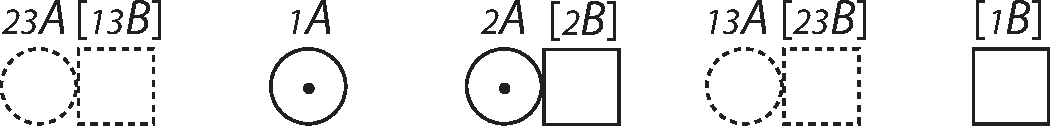
\includegraphics[width=0.56\textwidth]{gesamttex/edit_VIII-4/images/LH_35_14_02_040_d1_040r.pdf}%
\edcaption[0.75em]{%
\edtext{%
\lbrack\textit{Fig.\:1}\rbrack%
}{\lemma{\lbrack\textit{Fig.\:1}\rbrack}%
\Cfootnote[nonum]{%
Die im Diagramm vertauschten Bezeichnungen
\textit{\ind{13}B} und \textit{\ind{23}B}
sind sinngemäß geändert,
die fehlenden Bezeichnungen \textit{\ind{1}B} und \textit{\ind{2}B} ergänzt worden.%
}}%
}%
\vspace{2.25em}%
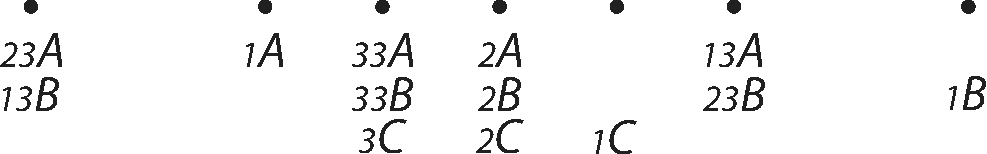
\includegraphics[width=0.52\textwidth]{gesamttex/edit_VIII-4/images/LH_35_14_02_040_d2_040r.pdf}%
\edcaption[0.75em]%
{%
\lbrack\textit{Fig.\:2}\rbrack%
}%
\end{edfigure}%
\pstart%
\noindent%
\edtext{%
Videamus an%
}{\lemma{}%
\Bfootnote{%
Videamus %
\bars{si corpora sint aequalia \textit{gestr.}} %
an%
~\textit{L}%
}}
res succedat,
ut possimus
\edtext{%
ponere corpus%
}{%
\lemma{}%
\Bfootnote{%
ponere %
\bars{utrumque \textit{gestr.}} %
corpus%
~\textit{L}%
}}
tam suo quam contrario nisu%
\indexS{nisus proprius}%
\indexS{nisus contrarius}%
\indexS{corpus latum nisu suo}%
\indexS{corpus latum nisu contrario}
ferri %
sic,
ut ponatur ferri illuc
ubi centrum est gravitatis amborum.%
\indexS{centrum gravitatis commune}
\edtext{%
Sit
\edtext{%
ipsius \textit{A}
}{%
\lemma{ipsius \textit{A}}%
\Cfootnote{Vgl. das Diagramm \lbrack\textit{Fig.\:2}\rbrack.}}%
directio et velocitas%
\indexS{directio in concursu}%
\indexS{velocitas in concursu}
\textit{\ind{1}A}\textit{\ind{2}A},%
}{%
\lemma{Sit}%
\Bfootnote{%
\textit{(1)}~\textit{A} %
\textit{(2)}~ipsius \textit{A} %
\textit{(a)}~conatus et %
\textit{(b)}~directio et~velocitas \textit{\ind{1}A}\textit{\ind{2}A},%
~\textit{L}%
}}
quae continuata esset in \textit{\ind{13}A},
et similiter sit ipsius \textit{B} velocitas
\textit{\ind{1}B}\textit{\ind{2}B},
continuata in \textit{\ind{13}B}.
Utique scimus
ita ferri centrum gravitatis%
\indexS{centrum gravitatis commune}
\edtext{%
commune \textit{C},
ut%
}{%
\lemma{}%
\Bfootnote{%
commune %
\bars{\textit{C} \textit{erg.}}, %
ut%
~\textit{L}}}
fuisset latum
si successum habuissent
\textit{\ind{13}A} et \textit{\ind{13}B}.
Itaque si contra daremus simul ipsi
\textit{A}
motum ipsius
\textit{B},
seu \textit{\ind{23}A},
et
\edtext{%
ipsi
\lbrack\textit{B}\rbrack\
motum ipsius
\lbrack\textit{A}\rbrack,
seu \textit{\ind{23}B},%
}{%
\lemma{}%
\Bfootnote{%
ipsi %
\bars{\textit{A} \textit{ändert Hrsg.}} %
motum ipsius %
\bars{\textit{B} \textit{ändert Hrsg.}}, %
seu \textit{\ind{23}B},%
~\textit{L}%
}}
\ledpb%
rursus idem erit progressus centri gravitatis%
\indexS{progressus centri gravitatis}%
\indexS{centrum gravitatis commune}
quia corpora sunt aequalia.%
\indexS{corpora concurrentia aequalia}
Itaque coincident
et \textit{\ind{33}A}, \textit{\ind{33}B} %
et \textit{\ind{3}C},
sed in inaequalibus%
\indexS{corpora concurrentia inaequalia}
non
\edlabel{35_14_02_040_1a}%
coinciderent.%
\edtext{}{%
\xxref{35_14_02_040_1a}{35_14_02_040_1b}%
\lemma{coinciderent.}%
\Bfootnote{%
\textit{(1)}~Sed fortasse sic procedere licebit, ut corpori %
\textit{(a)}~\textit{A} %
\textit{(b)}~uni %
\textit{(2)}~Sed an %
\lbrack\href{\Scan{LH_35_14_02_040v}}{40\,v\textsuperscript{o}}\rbrack\ \lbrack/\rbrack\ %
\textit{(3)}~\bars{Revera succedet \lbrack...\rbrack\ succedet compositio. \textit{erg.}} %
\lbrack\href{\Scan{LH_35_14_02_040r}}{40\,r\textsuperscript{o}}\rbrack\ %
\textit{(a)}~Eadem quantitas %
\textit{(b)}~Si corpus ducatur in %
\textit{(aa)}~omne %
\textit{(bb)}~aggregatum omnium %
\textit{(aaa)}~conatuum %
\textit{(bbb)}~velocitatum quas %
\lbrack...\rbrack\ 
in universo.%
~\textit{L}%
}}
\edlabel{35_14_02_040_2a}%
\lbrack%
\href{\Scan{LH_35_14_02_040v}}%
{40\:v\textsuperscript{o}}%
\rbrack%
\pend%
\pstart%
Revera succedet haec compositio %
si%
\lbrack,\rbrack\
ut res est,
ponamus
corpora concurrentia nisum%
\indexS{nisus dissiliendi}
semper habere a se invicem
reciprocis velocitatibus respectivis%
\indexS{velocitas respectiva}
dissiliendi%
\indexS{velocitas dissiliendi}
et praeterea motum communem%
\indexS{motus communis}
manere,
ut in navi%
\indexS{navis}
semper succedet
\edlabel{LH_35_14_02_040_40v/r_syyrtym-1}%
compositio.%
\indexS{compositio motuum}%
\edtext{}%
{\xxref{LH_35_14_02_040_40v/r_syyrtym-1}{LH_35_14_02_040_40v/r_syyrtym-2}%
\lemma{compositio. \lbrack/\rbrack\ Si corpus}%
\Cfootnote{In \textit{L} waagerechte Trennlinie zwischen den Absätzen.%
}}
\href{\Scan{LH_35_14_02_040r}}%
{\lbrack40\:r\textsuperscript{o}\rbrack}%
\pend%
\pstart%
\edlabel{LH_35_14_02_040_040r_aggregatum-1}%
Si%
\edlabel{35_14_02_040_1b}
corpus%
\edlabel{LH_35_14_02_040_40v/r_syyrtym-2}
ducatur%
\indexS{ductus corporis in aggregatum velocitatum}
in aggregatum omnium velocitatum%
\indexS{aggregatum velocitatum}
quas habuit inde a quiete%
\lbrack,\rbrack\
summa factorum in corpora%
\indexS{summa factorum in corpora}
erit eadem in
\edlabel{35_14_02_040_3a}%
universo.%
\indexS{universum}%
\edlabel{35_14_02_040_2b}%
\edlabel{LH_35_14_02_040_040r_aggregatum-2}%
\edtext{}{%
\xxref{35_14_02_040_3a}{35_14_02_040_3b}%
\lemma{universo. \lbrack/\rbrack\ Semper}%
\Cfootnote{%
In \textit{L} waagerechte Trennlinie zwischen den Absätzen.%
}}%
\pend%
\pstart%
Semper%
\edlabel{35_14_02_040_3b}
succedit compositio motuum.%
\indexS{compositio motuum}
Semper conservatur eadem potentia,%
\indexS{potentia conservata}
seu semper idem est
\edtext{%
effectus absolutus.%
\indexS{effectus absolutus}
Semper res ita prodeunt,
ut discerni nequeat
in quo corpore sit motus.%
}{%
\lemma{effectus}%
\Bfootnote{%
\bars{absolutus \textit{erg.}}. %
\textit{(1)}~Semper
\textit{(a)}~obtinetur %
\textit{(b)}~\textlangle idem est\textrangle\ effectus %
\textit{(c)}~eadem directio in summa %
\textit{(2)}~Semp %
\textit{(3)}~Semper %
\textit{(a)}~in %
\textit{(b)}~res ita %
\lbrack...\rbrack\ sit motus.%
~\textit{L}%
}}
\pend%
\pstart%
Duplex potentia in natura,%
\indexS{potentia duplex in natura}%
\indexS{natura}
una
\edtext{%
absoluta,%
\indexS{potentia absoluta}
ubi nihil interest%
}{%
\lemma{absoluta,}%
\Bfootnote{%
\textit{(1)}~nihil re %
\textit{(2)}~ubi nihil interest%
~\textit{L}%
}}
in quo
sit corpore,
altera conservativa%
\indexS{potentia conservativa}%
\lbrack,\rbrack\
qua conatur idem corpus
suam velocitatem et directionem retinere%
\indexS{conatus retinendi velocitatem}%
\indexS{conatus retinendi directionem}%
\lbrack,\rbrack\
et ab hac oritur percussio.%
\indexS{percussio}
Ab hac etiam oritur conatus%
\indexS{conatus alternativus}
\edtext{%
alternativus.
Et porro licet%
}{%
\lemma{alternativus.}%
\Bfootnote{%
\textit{(1)}~Et\textlangle iam\textrangle\ %
\textit{(2)}~Et porro licet%
~\textit{L}%
}}
\href{\Scan{LH_35_14_02_040v}}%
{\lbrack40\:v\textsuperscript{o}\rbrack} %
potentia conservativa%
\indexS{potentia conservativa}
in
\edtext{%
singulis exitum habere non possit,
habet tamen in summa plurium %
simul.%
}{%
\lemma{singulis}\Bfootnote{%
\textit{(1)}~conservari non possit, ta %
\textit{(2)}~exitum habere %
\lbrack...\rbrack\ plurium, simul.%
~\textit{L}%
}}
Hoc est%
\lbrack,\rbrack\
summa directionum%
\indexS{summa directionum}
semper succedit.
\pend%
\vspace{5em}%
\pstart%
\noindent%
\centering%
*    *    *
\pend%
\newpage%
\selectlanguage{ngerman}%
\begin{ledgroup}
\footnotesize
\pstart
\noindent%
\textls{Ausführliche Datierungsgründe:}%
\pagelabel{58235_dat}
Die titellose und undatierte Aufzeichnung N.\;\ref{58235} ist auf einem Träger überliefert, dessen römische\indexO{Rom} Herkunft sich durch Vergleiche mit weiteren Handschriften aus dem Leibniz-Nachlass feststellen lässt;
auf gleichem Papier sind auch die Aufzeichnungen N.\;\ref{58656-A}, N.\;\ref{58258} und N.\;\ref{58218} im vorliegenden Band verfasst worden (siehe für die Details die ausführliche Datierungsgründe zu N.\;\ref{58656-A}, S.\;\pageref{58656-A_dat}).
Bei all diesen Texten, von denen N.\;\ref{58656-A} und N.\;\ref{58258} auch einen inhaltlichen Zusammenhang mit Leibnizens \textit{Dynamica} aufweisen, %
ist demnach eine Entstehungszeit anzunehmen, die sich auf die Monate vom Sommer bis zum November 1689 erstrecket, als Leibniz in Rom\indexO{Rom} am \textit{Phoranomus}\cite{01402} und an der ersten Fassung der \textit{Dynamica}\cite{01354} gearbeitet hat (siehe \textsc{Robinet} 1988, S.\;81\,ff.).\cite{01240}
\pend%
\pstart%
Die Aufzeichnung N.\;\ref{58235} kann man nämlich als Beitrag zu der unvollendet gebliebenen Stoßlehre der \textit{Dynamica}\cite{01354} ansehen (siehe zur Entstehung der Abhandlung unter besonderer Berücksichtigung der Stoßlehre die einleitende Erläuterung zu den Entwürfen N.\;\ref{impulsuseccentricus} im vorliegenden Band, \refpassage{impulsecc_intro_Dynam-1}{impulsecc_intro_Dynam-2}).
In dieser Hinsicht ist Folgendes zu beachten:
Leibniz unterscheidet in seinen \textit{Dynamica}, pars~I, sectio~III, cap.\;II, def. zwischen absoluter und relativer Potenz: \textit{Distinguo autem potentiam mobilis \textls{absoluta,} in corpore per se consideratam, a \textls{respectiva,} qua aliud percutit, de qua suo loco} (%
\textit{CFP}~I, S.\;145.12--14~\bracks{A}; S.\;517.2--4~\bracks{B}; II.1,\;S.\;202.1--3~\bracks{C}).\cite{01354}
Die \glqq relative Potenz\grqq\ bzw. \glqq relative Kraft\grqq\ wird dann zunächst ebd., pars~II, sectio~I, \bracks{cap.\;II,} def.\;7 (\textit{Vis respectiva est, qua duo corpora in se invicem agunt}) und prop.\;41 u.\;42 untersucht, wobei die Stoßlehre auch dort den Rahmen festlegt (%
\textit{CFP}~I, S.\;349.12--352.17~\bracks{A}; S.\;585.28--588.17~\bracks{B}; II.2, S.\;426.13--430.31~\bracks{C}).\cite{01354}
Die Erhaltung der \glqq relativen Potenz\grqq\ wird vorwiegend ebd., pars~II, sectio~III, prop.\;7\textendash12 dargelegt (%
\textit{CFP}~I, S.\;400--412~\bracks{A}; %
II.2, S.\;498--512~\bracks{C}).\cite{01354}
Der Begriff \textit{potentia conservativa} wird dort nicht verwendet.
Das kann man als Zeichen dafür erachten, dass %
Leibniz bei der Bearbeitung der Stoßlehre der \textit{Dynamica}\cite{01354} den Begriff \textit{vis conservativa} aufgegeben und lediglich den Begriff \textit{vis respectiva} beibehalten hat.
Dies könnte wiederum zeigen, dass die Aufzeichnung N.\;\ref{58235} vor oder während der Bearbeitung der A-Fassung der \textit{Dynamica}\cite{01354} entstand und aus inhaltlichen Gründen beiseite gelegt wurde.%
\pend%
\pstart%
Die Aufzeichnung N.\;\ref{58235} ist demgemäß auf den Zeitraum zwischen Sommer und November 1689 zu datieren.
Eine frühere (ab Leibnizens Ankunft in Rom\indexO{Rom} im Mai 1689) oder eine spätere Abfassungszeit (höchstens bis Ende März 1690, als Leibniz Italien\indexO{Italien} verlassen hat) sind nicht ausgeschlossen, aber unwahrscheinlich.%
\pend%
\end{ledgroup}
\normalsize%
\selectlanguage{latin}%
\frenchspacing%
